\documentclass[12pt,a4paper]{book}
\usepackage{graphicx} 
\usepackage{multicol}
\begin{document}
	\title{RASD myTaxiService}
	\author{Marco Giuliano}
	\date{6 November 2015}
	\maketitle
	\tableofcontents
	\chapter{Introduction}
		\section{Purpose}
		This Requirements Analysis and Specification Document (RASD) is intended to describe the \textit{myTaxiService} system and define an agreement on expected functionalities, as specified on the contract, between both the customer and the supplier.
		\section{Scope}
		The project aims to develop a solution to optimize and manage the taxi service in the city customer.
		The solution should be composed of different modules, each with a specific function. The main component is the \textit{myTaxi\textunderscore Server}; this is the heart of the application, it stores data about taxis and customers and it manages the business logic for the correct operativity of the whole system.
		There should be also different front-end components: 2 for customers (\textit{myTaxi\textunderscore Web} and \textit{myTaxi\textunderscore Mobile}), one for the taxi driver (\textit{myTaxi\textunderscore Driver})and one for the city administration (\textit{myTaxi\textunderscore Administration}).
		\textit{myTaxi\textunderscore Web} and \textit{myTaxi\textunderscore Mobile} are used by the customers to reserve a taxi and receive and acknowledge message by the system communicating the estimated time of arrival of the car.
		\textit{myTaxi\textunderscore Driver} is the interface module in use of the taxi drivers, it enables them to receive calls by the customers and indication about the location they have to reach to pick the customer up.
		\textit{myTaxi\textunderscore Administration} is used by the administrator of the system: it enables them to add or remove taxi drivers and to monitor the state of the system.
		Overall this solution should increase the level of service provided by the city taxi's system both for customers and drivers: customers would be served more precisely and in shorter time and market share for drivers would be fairer because of the automated management of the queues.
			\subsection{Goals}
			Here the list of the goals of the myTaxiService application:
			\begin{itemize}
			 \item[\textbullet] [G.1] City Government can activate taxis into the system;
			 \item[\textbullet] [G.2] Every user in the city area can use the mobile application or the web application to reserve a taxi;
			 \item[\textbullet] [G.3] Every user, after reserving a taxi, receive an acknowledge by the system communicating the number of the incoming taxi and the ETA;
			 \item[\textbullet] [G.4] It is guaranteed a fair distribution of runs;
			 \item[\textbullet] [G.5] Drivers have the discretion to accept or refuse a call;
			 \item[\textbullet] [G.6] When a registered driver turns on the transponder the system automatically recognize the corresponding taxi as available to the service and inserts it in the corresponding queue based on its position;
			 \item[\textbullet] [G.7] When a registered driver turns off the transponder the system removes the corresponding taxi from the queue;
			 \item[\textbullet] [G.8] The system maintain a QoS of 90\% of users served in max 8 minutes;
			 \item[\textbullet] [G.9] In case of congestion of the system a message is promped to the user;
			\end{itemize}
		\section{Definitions, acronyms and abbreviations}
			\subsection{Definitions}
				\begin{itemize}
					\item[\textbullet] [User] They are considered the end-users of the myTaxiService application: people who need to reserve a taxi to travel in the city.
					\item[\textbullet] [Authorized Driver] They are the drivers of taxi with a regular license who are authorized to work in the city. They are the only one who can be inputed into the database of the myTaxiService system.
					\item[\textbullet] [Registered Taxi] Cars with a regular license, as stated by the law, that can be used by authorized drivers for the service.
					\item[\textbullet] [City Area] Zone in which the city is divided to better distribute cars and users in order to offer a better service and a fairer distribution of work between taxis.
					\item[\textbullet] [Mobile Application] It's a software to download on a mobile device. In our specific case it's a module of the system-to-be in use to the Users to make reservations of taxis.
					\item[\textbullet] [Transponder] A radio device that transmit an unique ID and a position to the server of the mmyTaxiService.
					\item[\textbullet] [Congestion of the system] A situation in which most of the taxi actually in service are busy.
					\item[\textbullet] [Internet] The global network for data transmission.
				\end{itemize}
			\subsection{Acronyms}
				\begin{itemize}
					\item[\textbullet][ETA] Estimated time on Arrival. It represents the estimated time, calculated by the system, that the user should wait until the incoming taxi will reach to pick him up.
					\item[\textbullet][FIFO] First In First Out. It is a methodology in queue management where the first element entered in a queue is the first element served.
					\item[\textbullet][RASD] Requirement Analysis and Specification Document. It is the document written to specify the requirements of a system to implement.
					\item[\textbullet][GUI] Graphic User Interface. It's an interface used by users to interact with a system.
					\item[\textbullet][LAN] Local Area Network. It'a local and private network for the transmission of data.
				\end{itemize}
			\subsection{Abbreviations}
				\begin{itemize}
					\item[\textbullet] [App] Abbreviation used to indicate a mobile application.
					\item[\textbullet] [Ack] Abbreviation used to indicate an acknowledge message.
					\item[\textbullet] [Driver] Used in this document to indicate an Authorized Driver
					\item[\textbullet] [Taxi] Used in this document to indicate a Registered Taxi
					\item[\textbullet] [Run] Used in this document to indicate a service of transport made by a Taxi for an User
					\item[\textbullet] [G.\textit{n}] Goal number "n"
					\item[\textbullet] [D.\textit{n}] Domain property number "n"
					\item[\textbullet] [R.\textit{n}] Requirement number "n"
				\end{itemize}
		\section{References}
			\begin{itemize}
				\item[\textbullet] Specification document \textbf{Assignments 1 and 2 (RASD and DD).pdf} for the project \textit{myTaxiService}
				\item[\textbullet] IEEE Std 830-1998 \textbf{IEEE Standard For Requirement Specification.pdf}
				\item[\textbullet] National, regional and local laws and regulamentation about public transportation and rent of cars with driver;
			\end{itemize}
		\section{Overview}
			This RASD document will be organized, as the standard IEEE 830-1998 suggest, in four different parts:
			\begin{itemize}
				\item[\textbullet] [Introduction]
				\item[\textbullet] [Overall Description]
				\item[\textbullet] [Specific Requirements]
				\item[\textbullet] [Appendix]
			\end{itemize}
	\chapter{Overall Description}
	This chapter will describe how the system to be developed will be integrated with the actual environment, how it will interact with the stakeholders and which are the assumptions to be made before specifying the requirements that it must satisfy.
		\section{Product perspective}
		The myTaxiService system will be the only technology application in use to the city for the management of the taxi service. It won't need to be inegrated with any other existing product.
			\subsection{System interfaces}
			The system should provide an API that exposes the main services used for reservation (the same used by the Mobile and Web module). This interface will be used by developers to provide in the future further services based on the myTaxiService such as taxi sharing or advanced reservation.
			\subsection{User interfaces}
			As mentioned before, the system will provide four different kind of user interfaces: two are destinated for the Users, one for the drivers and one for the city administration.
			The two interfaces for Users (web and mobile) must be easy to use: no more than one message at time should be provided on the screen and no more than a double choiche should be asked (all requests should be composed with the "Yes/No" pattern).
			The taxi's interface should be developed for a 11 inch monitor (the monitor will be integrated on the dashboard) and the information showed on the screen should be limited in order to keep the use of a big font to avoid the distraction of the drivers.
			The administrator's interface should contain every information about the current situation of the system such as incoming calls, busy taxis, available taxis, state of the queue of every zone and list of authorized taxis.
			\subsection{Hardware interfaces}
			The system should provide an interface to the navigation system of the taxis, to help drivers to transfer GPS data of the destination to their own navigation system.
			The User interface module should work only if authorized to use the GPS sensor of the device where is installed (and, of course, the GPS sensor must be present).
			\subsection{Software interfaces}
			The system should provide internal interfaces for the different modules that are going to be implemented: every GUI module should be able to communicate with the server using specific services provided by this.
			\subsection{Communications interfaces}
			The main communication interface is the Internet. Mobile, Web and Driver's module will use it for information exchange with the Server. The Administrator's interface communicates with the server using the LAN of the City Government.
			\subsection{Memory contraints}
			The system shouldn't need to access the memory of Users devices.
			The system should need to access the memory of Drivers devices to store data about the next serving User.
			Data of Users, Drivers and runs should be stored on a permanent memory on the Server for at least 5 years for statistical research.
		\section{Product functions}
		The system will provide the following functions for each category of end user
			\subsection{City Government}
				\begin{itemize}
					\item[\textbullet] Add a Taxi to the list of the registered Taxis
					\item[\textbullet] Remove a Taxi from the list of the registered Taxis
					\item[\textbullet] Inquiry the system about the status of the taxi service (number of busy cars, number of free cars, number of waiting customers, number of served customers)
				\end{itemize}
			\subsection{Driver}
				\begin{itemize}
					\item[\textbullet] Join the queue of the corresponding zone as a registered taxi turning on the transponder
					\item[\textbullet] Leave the queue of the corresponding zone as a registered taxi turning off the transponder
					\item[\textbullet] Receive an incoming call
					\item[\textbullet] Accept an incoming call
					\item[\textbullet] Refuse an incoming call
					\item[\textbullet] Signal that the User is on board and the run has bagun
					\item[\textbullet] Signal that the User left the car and the run has ended
				\end{itemize}
			\subsection{User}
				\begin{itemize}
					\item[\textbullet] Download the app
					\item[\textbullet] Get authenticated into the system
					\item[\textbullet] Reserve a taxi
				\end{itemize}
		\section{User characteristics}
		The typical users of the system shouldn't necessary have a technology background. The only required competency is a certain familiarity with modern technology, touchscreens and mobile phone / tablet.
		In addition, drivers should be trained in the use of the \textit{myTaxi\textunderscore Driver} module and the city government's user should be trained in the use of \textit{myTaxi\textunderscore Administration} module for their peculiarities.
		\section{Constraints}
		The functional analysis and the development phases of the project may be subject to the following constraints:
			\subsection{Regulatory policies}
			All the studies and the implementations should be subject to the national, regional and local laws in the field of public transportaion and renting of cars with driver.
			\subsection{Hardware limitations}
			The following hardware limitations should be considered in the design phase:
			\begin{itemize}
				\item[\textbullet] Mobile network availability for the Users and the Drivers;
				\item[\textbullet] Computational capacity in order to allow a real time dispatching of calls under the condition of the maximum number of taxi in service
				\item[\textbullet] Issues retrieving the position with the GPS sensor in use of the Users
			\end{itemize}
			\subsection{Interfaces to other applications}
			It should be possible to transmit the position of the User to serve from the Driver module to the GPS navigation system installed on the taxi. The analyst should consider an interface compatible to all the navigation system installed on the cars.
			\subsection{Parallel operations}
			It should be considered, in the analysis phase, that in the peak hours the system could receive an average of 20 calls every minute.
			\subsection{Higher-order language requirements}
			Consider the use of a common programming language in order to encourage external developers to use APIs and improve with new functions the system.
			\subsection{Signal handshake protocols}
			Every operation made by a user should receive an answer by the system considering the use of mobile radio network.
			\subsection{Reliability requirements}
			A taxi should be always driven at the correct destination. User that received and ack shouldn't wait an indefinite time because the driver can't find them.
			Every run should be traced and monitored by the city administration.
			\subsection{Safety and security considerations}
			Consider, during the analysis phase, a metodology to make the Driver's module compatible to a safe guide.
		\section{Assumptions and dependencies}
			\subsection{Assumptions}
			The following assumption should be considered before formalizing the requirements:
			\begin{itemize}
				\item[\textbullet] When a user reserves a taxi it's sure that he needs it and he will be waiting at the place from where he made the reservation;
				\item[\textbullet] There is always an available route between the taxi and the calling User;
				\item[\textbullet] Taxis and Users are equally distributed between the zones;
				\item[\textbullet] Every time a taxi begins a run with a passenger it will bring the User to the destination required. A run can't be interrupted.
				\item[\textbullet] Coordinates comunicated by the User's app are always correct
				\item[\textbullet] If a run ends in a zone different than the origin then the taxi will enter the queue of the new zone;
			\end{itemize}
		\section{Apportioning of requirements}
		Many possible improvement could be considered for further versions of the product, such as:
		\begin{itemize}
			\item[\textbullet] The possibility to cancel a reservation by the User;
			\item[\textbullet] The possibility, for the City Administration, to suggest a Driver to relocate his taxi in a different zone considering the amount of calls received and the lenght of taxi's queues;
			\item[\textbullet] The possibility, for a Driver, to freeze his position in queue for a certain amount of time in order to take a break avoiding the possibility to jump to the end of the queue;
			\item[\textbullet] The possiblity to pay the run with the mobile app at the end of it;
			\item[\textbullet] The possibility to specify the destination of the run at the moment of the reservation in order to improve the route calculation engine and optimize the use of the taxi and the queue;
		\end{itemize}
	\chapter{Specific Requirements}
		\section{External interfaces}
		To list the External interfaces of the system it should be important to distinguish between interfaces with external stakeholders and interfaces between internal modules. There are 2 kind of interfaces between external stakeholders:
		\begin{itemize}
			\item[\textbullet] GUIs;
			\item[\textbullet] APIs;
			\item[\textbullet] External DBMS; description
		\end{itemize}
		Interfaces between internal components are the following:
		\begin{itemize}
			\item[\textbullet] Wired network;
			\item[\textbullet] Mobile radio network;
			\item[\textbullet] Software (OS and internal DBMS);
		\end{itemize}
			\subsection{User Interfaces}
				\paragraph{Administrator's Interfaces}
				\hfill\break
				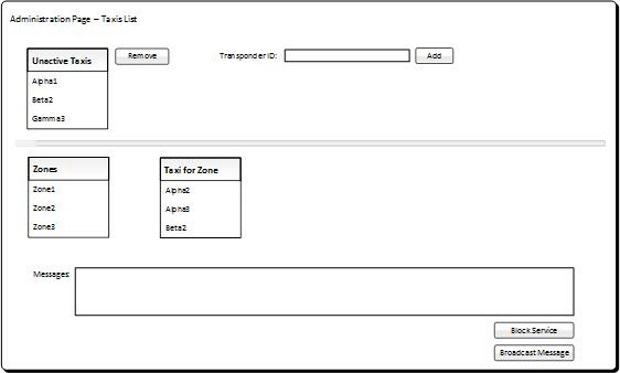
\includegraphics {admin_page}
				\paragraph{Driver's Interfaces}
				\hfill\break
				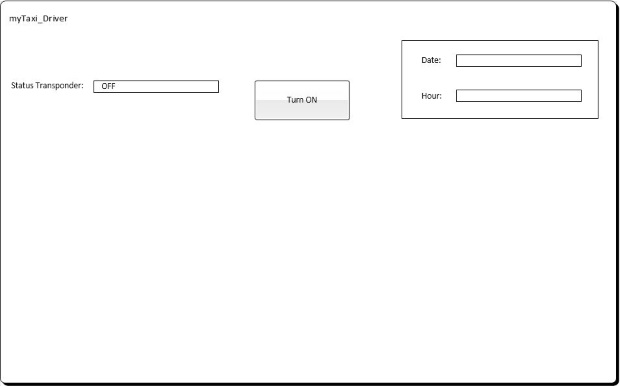
\includegraphics {driver_page1}
				\hfill\break
				This interface is shown when the transponder is turned off and the taxi is not in service (not in the queue). This give the possibility to turn on the transponder and join the queue of taxis in service.
				\hfill\break
				\hfill\break
				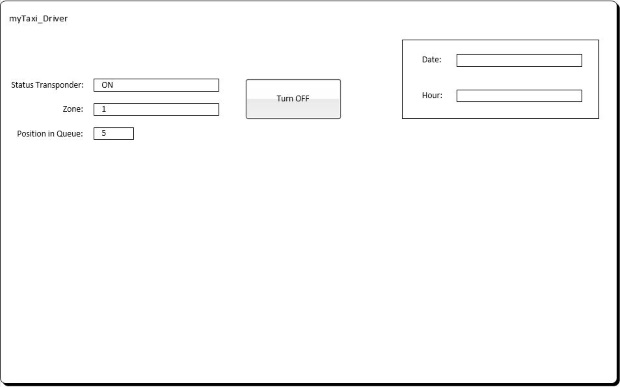
\includegraphics {driver_page2}
				\hfill\break
				This interface is shown when the driver turns on the transponder. It shows the zone in which the taxi is (depending on the position measuded by the GPS sensor) and the position in the corresponding queue. It gives the possibility to turn off the transponder and leave the service.
				\hfill\break
				\hfill\break
				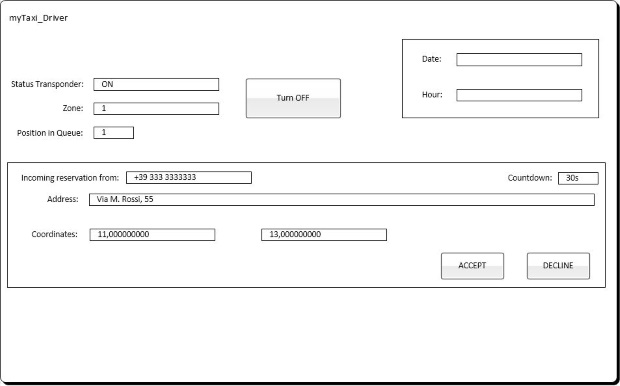
\includegraphics {driver_page3}
				\hfill\break
				This interface is shown when the taxi receives an incoming call. It signals informmation about the calling User (ID, address and position) and gives the possibility to accept or decline the call.
				\hfill\break
				\hfill\break
				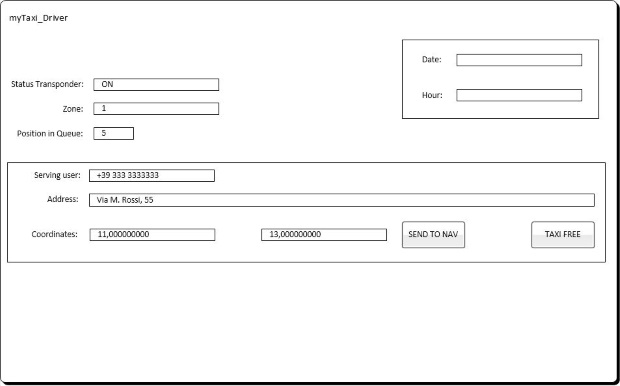
\includegraphics {driver_page4}
				\hfill\break
				This interface is shown if the driver accepts the incoming request. It shows information about the serving User, it gives the possibility to send information about the position  to the car navigator and the possibility to communicate the end of the run (to rejon the queue). During the service there's not the possibility to turn off the transponder.
				\paragraph{Users' Interfaces}
				\hfill\break	
				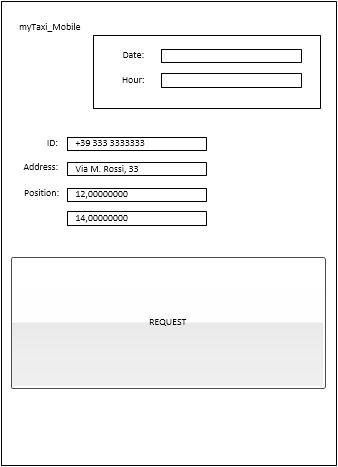
\includegraphics {mobile_page1}
				\hfill\break
				This is the main interface of the myTaxi\textunderscore Mobile. When opened it shows information about the logged user and the position. It offers the possibility to reserve a taxi.
				\hfill\break
				\hfill\break	
				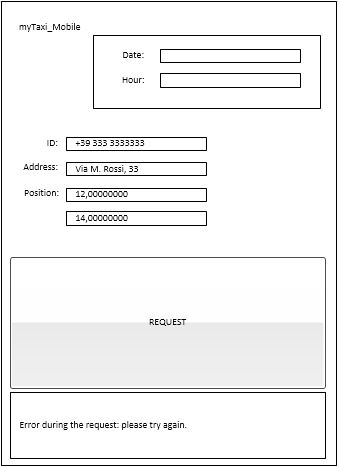
\includegraphics {mobile_page2}
				\hfill\break
				This screen is shown if, after trying to reserve a taxi, an error has occurred.
				\hfill\break
				\hfill\break	
				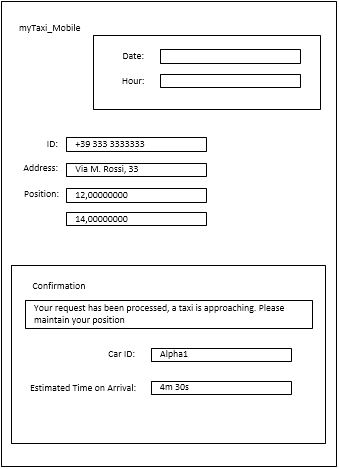
\includegraphics {mobile_page3}
				\hfill\break
				This screen is shown after a reservation is made. It shows the ID of the incoming taxi and the estimated time on arrival. At this point the user can close the application.
			\subsection{APIs}
			The system should expose every function used to reserve a taxi using an API to allow external programmer to develop new functionalities based on the core of the system. Functionalities about the administration panel and the Driver's interface should remain hidden in exclusive use of the city government and his supplier.
			\subsection{External DBMS}
			The system should be able to connect to the Database, managed by the city, containing the list of all licensed taxis.
			\subsection{Wired Network}
			The server hosting the application should reside in the LAN of the City Government. The administration module should be connected by this LAN to the application core.
			The application server should be connected, by a wired Internet connection, to the three main mobile providers in order to reach every possible user and driver connected by a mobile network.
			\subsection{Mobile Radio Network}
			User's and Driver's modules should connect to the application core using a mobile radio network. This interface should allow the transmission of small packet (maximum 16kb of data at time).
			Availability of the network must be guarantee only during the reservation and acceptance phases. After that the system can work "offline".
			\subsection{Software (OS and DBMS)}
			There are not specific requirements for OS. The system should work on any platform in commerce for mobile devices and on any OS for the application server.
			The DBMS should be transactional and should manage autonomously read/write concurrency. One of the most common commercial packages should work fine for our purpose.
		\section{Functions}
			\subsection{[G.1] City Government can activate taxis into the system}
			\begin{itemize}
				\item[\textbullet] [D.1] Only authorized users can log into the system with privileges provided to the "City Government";
				\item[\textbullet] [D.2] There is a list in a Database of the City government containing all the taxis with a regular license;
				\item[\textbullet] [R.1] The taxi to be added should have a tablet device where to install the Driver's module and it should be connected to the GPS system and the transponder;
				\item[\textbullet] [R.2] When activated into the system, a taxi should be inserted into the list of authorized Taxis with a specific ID (the transponder ID);
				\item[\textbullet] [R.3] When an administrative user activates a taxi into the system the operation should be logged indicating which user did it, the date, the hour of the operation and the taxi's ID activated;
			\end{itemize}
			\subsection{[G.2] Every user in the city area can use the mobile application or the web application to reserve a taxi}
			\begin{itemize}
				\item[\textbullet] [D.1] The User has the app installed on his mobile device or opens the web page on his browser;
				\item[\textbullet] [D.2] The app or the website are authorized to retrieve the mobile phone number and to use it as unique ID of the User;
				\item[\textbullet] [D.3] The position of the User is retrieved using the GPS sensor installed on his mobile device;
				\item[\textbullet] [R.1] When a User makes a reservation, a data packet is sent to the system indicating the exact position, the date and the hour of reservation;
				\item[\textbullet] [R.2] In case of absence of radio network the User's module should wait for 30 seconds and try to send another packet;
				\item[\textbullet] [R.3] After 4 try (2 minutes) a message should appear on the User's device to alert that the request has not been sent due to absence of radio signal;
				\item[\textbullet] [R.4] When the request is received by the system an ack message should be sent to the User's device. This message makes the User on hold;
			\end{itemize}
			\subsection{[G.3] Every user, after reserving a taxi, receive an acknowledge by the system communicating the number of the incoming taxi and the ETA}
			\begin{itemize}
				\item[\textbullet] [D.1] The User doesn't change his position after a reservation request is sent;
				\item[\textbullet] [D.2] The User doesn't close the App or the website on his device until he receives the notification of acceptance of the reservation;
				\item[\textbullet] [R.1] When a request reaches the system the server calculates which taxi should serve the request and the time spent to reach the customer using algorithms based on history;
				\item[\textbullet] [R.2] A message is sent from the server to the User's device communicating the ID of the taxi and the ETA;
				\item[\textbullet] [R.3] Data received by the User's device are visualized on the display and an ack message is sent from the User's device to the server;
			\end{itemize}
			\subsection{[G.4] It is guaranteed a fair distribution of runs}
			\begin{itemize}
				\item[\textbullet] [D.1] Every taxi has a position in the queue of taxis for a certain zone;
				\item[\textbullet] [R.1] The incoming reservation for a certain zone is assigned to the first taxi in queue for that zone;
				\item[\textbullet] [R.2] The taxi that received the last reservation request jumps to the last position of the queue;
			\end{itemize}
			\subsection{[G.5] Drivers have the discretion to accept or refuse a call}
			\begin{itemize}
				\item[\textbullet] [D.1] The reservation call is received by the taxi in the first position of the queue;
				\item[\textbullet] [R.1] The Driver's display show the address of the incoming call and a countdown timer indicating 30 seconds;
				\item[\textbullet] [R.2] 2 Big buttons occupies the lower half of the screen indicating "accept" or "refuse";
				\item[\textbullet] [R.4] If the countdown ends until the driver made his choiche, "refuse" is automatically chosen; 
				\item[\textbullet] [R.5] The choiche of the driver is sent to the system;
			\end{itemize}
			\subsection{[G.6] When a registered driver turns on the transponder the system automatically recognize the corresponding taxi as available to the service and inserts it in the corresponding queue based on its position}
			\begin{itemize}
				\item[\textbullet] [D.1] Every taxi has a transponder with an unique ID;
				\item[\textbullet] [R.1] When the driver turns on the transponder a radio signal is sent to the server with the ID and the actual position;
				\item[\textbullet] [R.2] When the server receives the "activation" signal checks that the taxi is registered into the system;
				\item[\textbullet] [R.3] If the taxi is registered is inserted in the last position of the queue of the zone corresponding the actual position of the taxi;
				\item[\textbullet] [R.4] If the ID is not present in the list of registered taxis then is ignored;
			\end{itemize}
			\subsection{[G.7] When a registered driver turns off the transponder the system removes the corresponding taxi from the queue}
			\begin{itemize}
				\item[\textbullet] [D.1] Every taxi has a transponder with an unique ID;
				\item[\textbullet] [R.1] When the taxi turns off the transponder the ID is sent to the server;
				\item[\textbullet] [R.2] When the server receives the ID of the turning off taxi, the car is removed from the corresponding queue;
			\end{itemize}
			\subsection{[G.8] The system maintain a QoS of 90\% of users served in max 8 minutes}
			\begin{itemize}
				\item[\textbullet] [D.1] The number of taxis is limited;
				\item[\textbullet] [D.2] The number of requests is potentially much larger than the number of taxis
				\item[\textbullet] [R.1] When the number of busy taxis reaches the 90\% in the majority of the zones an alert should be sent to the city administration;
			\end{itemize}
			\subsection{[G.9] In case of congestion of the system a message is promped to the user}
			\begin{itemize}
				\item[\textbullet] [R.1] The city government has the discrection to send a broadcast message to all the Users informing that a congestion of the service happened;
				\item[\textbullet] [R.2] The city government has the discrection to block any possible new reservation until the QoS is back to an acceptable level;
			\end{itemize}
		\section{Performance requirements}
		In general, the system should work with real time interaction. The designer should consider an amount of 200 cars, an average number of Users of 3000 each day.
		Every request made by a User should receive an answer, even if the connection with the server isn't available as previoulsy specified in the requirements.
		If an exception is raised by the application it should be notified to the users, giving them the possibility to make another reservation.
		\section{Logical database requirements}
		The system should log every operation made by every function already detailed in this document for a period of 5 year, for statistical purposes; 
		\section{Software system attributes}
			\subsection{Reliability}
			The system should allow every time a taxi accepts a reservation to make it reach the corresponding User.
			The User shouldn't wait for an indefinite time until a taxi serves his request if he receives the ack message;
			\subsection{Availability}
			The system should be available 99,5\% of the time every year. Downtime for maintenance, for the rest of the time, should be always scheduled in the nighttime between 3am and 4am;
			\subsection{Security}
			Informations on the mobile radio network should be encrypted;
			It should be impossible to log into the system as a Driver without a recognized transponder ID;
			\subsection{Maintainability}
			The interaction between modules should be guaranteed by webservices so that every module follows a mainteinance and versioning autonomous path;
			\subsection{Portability}
			The mobile modules should be multi-platform. They should be developed for iOS, Android and WP8.
	\chapter{Appendix}
		\section{UML Models}
			\subsection{Use Cases}
			\hfill\break	
			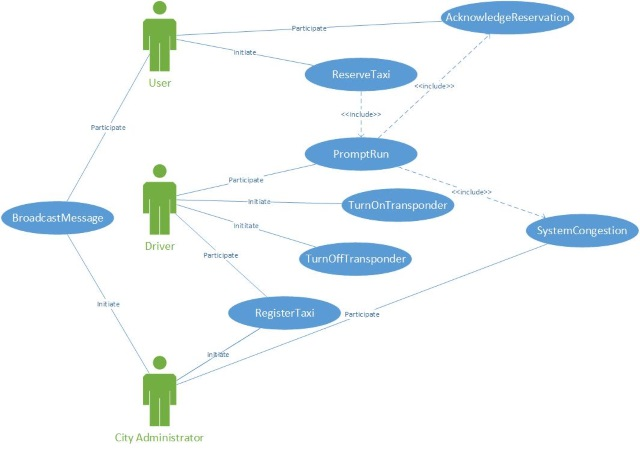
\includegraphics {USECase}
			\hfill\break
			\paragraph{RegisterTaxi}
			\begin{itemize}
				\item[\textbullet] [Actors] City Administrator (initialize), Driver
				\item[\textbullet] [Exceptions] The taxi isn't present in the DB of licensed cars;
				\item[\textbullet] [Flow of Events]
				\begin{itemize}
					\item[1] The administrator write in the textbox the code of the taxi
					\item[2] The systems accepts the code and write a record in the db
				\end{itemize}
				\item[\textbullet] [Special requirements] The taxi should be present in a specific DB
			\end{itemize}
			\paragraph{TurnOnTransponder}
			\begin{itemize}
				\item[\textbullet] [Actors] Driver (initialize)
				\item[\textbullet] [Exceptions] The taxi has not been registered in the system. The taxi is already in service.
				\item[\textbullet] [Flow of Events]
				\begin{itemize}
					\item[1] The Driver push the button on the main screen of the Driver's module
					\item[2] A radio message is sent to the server with an ID and a position.
					\item[3] The server checks if the ID is present in the database;
					\item[4] The server computes the zone in which the car is and calculates the position in the queue;
					\item[5] A message is returned to the taxi with the position in the queue
				\end{itemize}
				\item[\textbullet] [Special requirements] The taxi should be present in the system's db. The taxi should be not in service.
			\end{itemize}
			\paragraph{TurnOffTransponder}
			\begin{itemize}
				\item[\textbullet] [Actors] Driver (initialize)
				\item[\textbullet] [Exceptions] The taxi is not in service
				\item[\textbullet] [Flow of Events]
				\begin{itemize}
					\item[1] The Driver push the button on the main screen of the Driver's module
					\item[2] A radio message is sent to the server with an ID;
					\item[3] The server checks if the taxi isn't serving any User;
					\item[4] The server acknowledge to the taxi;
				\end{itemize}
				\item[\textbullet] [Special requirements] The taxi should be in service. The taxi shouldn't be serving any User.
			\end{itemize}
			\paragraph{ReserveTaxi}
			\begin{itemize}
				\item[\textbullet] [Actors] User (initialize)
				\item[\textbullet] [Exceptions] No mobile radio available. Impossible to retrieve the position
				\item[\textbullet] [Flow of Events]
				\begin{itemize}
					\item[1] The User opens the app
					\item[2] The user push the button to reserve a taxi
					\item[3] The system receives the message with the ID and the position of the User
					\item[4] The system checks if there is a free taxi in the corresponding zone;
					\item[5] The system assign a taxi to the service and executes the "PromptRun" function;
				\end{itemize}
				\item[\textbullet] [Special requirements] Mobile radio should be available. GPS position retrievable.
			\end{itemize}
			\paragraph{PromptRun}
			\begin{itemize}
				\item[\textbullet] [Actors] Driver
				\item[\textbullet] [Exceptions] No mobile radio available.
				\item[\textbullet] [Flow of Events]
				\begin{itemize}
					\item[1] A message appear on the Driver's device communicating information about a User.
					\item[2] The Driver accept or refuse the run
					\item[3] The choice is sent to the system
					\item[4] If the driver don't make any choice the run is automatically refused after 30 seconds
				\end{itemize}
				\item[\textbullet] [Special requirements] Mobile radio should be available.
			\end{itemize}
			\paragraph{AcknowledgeReservation}
			\begin{itemize}
				\item[\textbullet] [Actors] User
				\item[\textbullet] [Exceptions] No mobile radio available.
				\item[\textbullet] [Flow of Events]
				\begin{itemize}
					\item[1] The system calculates the route between the accepting taxi and the User
					\item[2] The system send a message to the User communicating the incoming taxi and the ETA
					\item[3] The message is displayed on the User's device
				\end{itemize}
				\item[\textbullet] [Special requirements] Mobile radio should be available.
			\end{itemize}
			\paragraph{SystemCongestion}
			\begin{itemize}
				\item[\textbullet] [Actors] City Administrator
				\item[\textbullet] [Exceptions] None
				\item[\textbullet] [Flow of Events]
				\begin{itemize}
					\item[1] The system calculates that less than 10\% of taxis are available
					\item[2] The system prompt a message on the administrator's interface
				\end{itemize}
				\item[\textbullet] [Special requirements] None
			\end{itemize}
			\paragraph{BroadcastMessage}
			\begin{itemize}
				\item[\textbullet] [Actors] City Administrator (initiate), User
				\item[\textbullet] [Exceptions] No mobile radio available
				\item[\textbullet] [Flow of Events]
				\begin{itemize}
					\item[1] The city administrator push a button on his interface indicating to broadcast a message
					\item[2] The message is broadcasted to all active users indicating that the service is temporary suspended due to a congestion
				\end{itemize}
				\item[\textbullet] [Special requirements] Mobile radio network should be available
			\end{itemize}
	\chapter{Revision}
	This is the first revision of the document. All the sections as is are written in the first version.
\end{document}